\section{Evaluation}
\label{sec.evaluation}

%In order to evaluate Lind's effectiveness in providing kernel protection, we
%conducted a series of experiments designed to answer four fundamental questions:

In order to evaluate Lind's effectiveness in containing untrusted code and
protecting OS kernel, we conducted a series of experiments to answer
four fundamental questions:

\textit{How does Lind compare to other virtualization systems
in protecting against historical Linux kernel bugs?}
(Section~{\ref{Linux-Kernel-Bug-Test-and-Evaluation}})
\yiwen{I am wondering if we should say ``zero-day bugs'' instead of ``historical bugs''.}

\textit{How much of the underlying kernel code is exposed, and is thus
vulnerable in different virtualization systems?}
(Section~{{\ref{Reachable-Kernel-Trace-Analysis-for-Different-Virtualization-Systems}})
%\yiwen{This question may need to be refined. Why is the question important to the readers?
%What is the take-away? The reachable kernel paths reflect an important security property
%of the system design. We want to express this point.}
%\lois{I made an attempt
%here at addressing your concerns. I agree its an important point to emphasize correctly.
%We might need to tweak it a bit more.}

\textit{If Lind's SafePOSIX reimplementation has bugs, how much of a threat does this pose?}
(Section~{{\ref{Reachable-Kernel-Trace-Analysis-for-Repy-Sandbox}})

\textit{In the Lind prototype, what is the expected overhead in
real-world applications?}
(Section~{{\ref{Performance-Evaluation}})

This section describes the setup of our experiments, 
and shows our experiment results. 
%and argues how the results support the merits of our secure design and its Lind prototype.
%\yiwen{If we claim the above sentence, then we need to say more about our secure design,
%which can be hard. Possibly remove ``our secure design'' and just keep ``Lind
%prototype.''}
%\lois{There might be some value to keeping the phrase in, since we
%are emphasizing the design and not the product.}
%
%\subsection{Experiment Methodology}
%
Our evaluation strategy was to directly compare the performance of Lind
against
seven other existing virtualization systems\textendash VirtualBox, VMWare
Workstation,
Docker, LXC, QEMU, KVM and Graphene. 
\yiwen{Should we talk about why we choose those systems and give some background information 
about them to readers who might not be familiar with some of them? 
It might be useful to state that we did pick up those systems in a systematic way.}
We also compared it against Native Linux as a baseline for comparison. 
%Because Native Linux is the original OS,
%without virtualization and additional protection, this data helps to
%clarify the security benefits of Lind,
%as well as whatever performance overhead costs the system may incur.


%\subsection{Experimental Setup, Results and Analysis}

%As dictated by the study questions listed above, our tests were conducted
%and appraised primarily from a security perspective
%(Section~{{\ref{Linux-Kernel-Bug-Test-and-Evaluation}} --
%%\S{\ref{Reachable-Kernel-Trace-Analysis-for-Different-Virtualization-Systems}},
%Section~{{\ref{Reachable-Kernel-Trace-Analysis-for-Repy-Sandbox}}).
%However, to get some idea of its potential efficacy
%in real-world settings, we also measured and evaluated the performance
%overhead of Lind
%(Section~{{\ref{Performance-Evaluation}})

\subsection{Linux Kernel Bug Test and Evaluation}
\label{Linux-Kernel-Bug-Test-and-Evaluation}

\textbf{Setup.}
To evaluate how well each virtualization system protect the Linux kernel against 
reported zero-day bugs, we identified and examined a list of  69 historical bugs that have
specifically targeted Linux kernel 3.14.1 \cite{CVE-Datasource}. 
By analyzing security kernel patches for those bugs,
we identified the lines of code in the kernel that correspond to each one. 

In order to test if a bug can be triggered, we created or located C
code capable of exploiting each of the kernel bugs \cite{Exploit-Database}.
We were only able to trigger and obtain results for 35 out of the 69 bugs in our experiments, 
either because of a difficulty in clearly determining if triggering had occurred, or an inability,
at this time, to find code to trigger them. We decided to focus our study on
only these bugs and leave the other, more complex ones, to future work and analysis.

We compiled and ran the exploit C code under each virtualization system to
obtain their kernel traces, and then used our kernel trace safety metric to
determine if a specific bug was triggered.

%\lois{I think this whole first paragraph can come out. All this information has
%been stated already. This is an evaluation of the RESULTS}
%We attempted to
%trigger 35 identified Linux kernel bugs by running programs in
%Native Linux, VirtualBox, VMWare Workstation, Docker, Graphene,
%and Lind.
%The kernel bugs examined are capable of causing serious security problems.
%For example,the CVE-2014-8989 bug allows local users to bypass intended file
%permissions by leveraging a POSIX ACL.
%The potential risk of triggering these and other types of
%kernel bugs when running applications, is a problem that
%needs to be taken seriously.

\noindent
\textbf{Results.}
We found that a substantial number of bugs could be triggered in existing
virtualization systems, as shown in Table \ref{table:trigger_vulnerabilities}.
A full 35 out of 35 (100\%) bugs were triggered in Native Linux,
while the other programs had lower rates: 14/35 (40\%) in
VirtualBox,
11/35 (31.4\%)  in VMWare Workstation, 8/35 (22.9\%)  in Docker,
12/35 (34.3\%)  in LXC, 5/35 (14.3\%)  in QEMU, 5/35 (14.3\%)  in KVM,
and 8/35 (22.9\%) bugs in Graphene.
In comparison, only 1 out of 35 bugs  (2.9\%) was triggered in Lind.

To better understand these results, 
%and particularly why Lind's performance was so strong, 
we take a closer look at four
vulnerabilities from Table \ref{table:trigger_vulnerabilities}. These short case
studies show how different system design philosophies can have 
different security impacts.
\yiwen{The following analysis needs to be refined. 
I need to rework with more information about the system call paths.}

\begin{table*}[!ht]
\scriptsize
\centering

\caption {\small Linux Kernel Bugs, and Vulnerabilities in Different Virtualization Systems
({\color{red}\ding{51}}: vulnerability triggered;
{\color{blue}\ding{51}}: vulnerability triggered with Guest Additions; \ding{55}: vulnerability
not triggered).}

%\resizebox{0.68\textwidth}{!}{\begin{minipage}{\textwidth}

\begin{tabular}{|p{1.7cm}|l|l|p{1cm}|p{1cm}|p{.8cm}|p{1cm}|p{.8cm}|p{1cm}|p{.8cm}|}\hline

\multirow{2}{1.7cm}{\bf Vulnerability}    &  \multirow{2}{.7cm}{\bf Native Linux}  &  \multirow{2}{*}{\bf VirtualBox}
&  \multirow{2}{.7cm}{\bf VMWare}
 & \multirow{2}{1cm}{\bf Docker} & \multirow{2}{1cm}{\bf LXC} &
\multirow{2}{1cm}{\bf QEMU} & \multirow{2}{1cm}{\bf KVM} &
\multirow{2}{1cm}{\bf Graphene} & \multirow{2}{1cm}{\bf Lind} \\ 
& & & & & & & & & \\
\hline

 CVE-2015-5706 & \multirow{1}{.7cm}{{\color{red}\ding{51}}} & {\color{blue}\ding{51}} &
\multirow{1}{1cm}{{\color{blue}\ding{51}}} & \multirow{1}{1cm}{{\color{red}\ding{51}}} & 
\multirow{1}{1cm}{{\color{red}\ding{51}}} & \multirow{1}{1cm}{{\color{red}\ding{51}}} & 
\multirow{1}{1cm}{{\color{red}\ding{51}}} & \multirow{1}{1cm}{{\color{red}\ding{51}}} & 
\ding{55}  \\

 CVE-2015-0239 & \multirow{1}{.7cm}{{\color{red}\ding{51}}} & {\color{red}\ding{51}} &
\multirow{1}{1cm}{{\color{red}\ding{51}}} & \ding{55} & \multirow{1}{1cm}{{\color{red}\ding{51}}} &
\multirow{1}{1cm}{{\color{red}\ding{51}}} & \multirow{1}{1cm}{{\color{red}\ding{51}}} &
 \ding{55}  & \ding{55}  \\
 
 CVE-2014-9584 & \multirow{1}{.7cm}{{\color{red}\ding{51}}} & \ding{55}  &
 \ding{55}  & \ding{55} & \ding{55} &
 \ding{55}& \ding{55} &
 \ding{55}  & \ding{55}  \\
 
 CVE-2014-9529 & \multirow{1}{.7cm}{{\color{red}\ding{51}}} & {\color{red}\ding{51}}  &
\ding{55}  & \ding{55} & \multirow{1}{1cm}{{\color{red}\ding{51}}} &
\ding{55}& \ding{55} &
\ding{55}  & \ding{55}  \\

 CVE-2014-9322 & \multirow{1}{.7cm}{{\color{red}\ding{51}}} & {\color{red}\ding{51}}  &
\ding{55}  & \multirow{1}{1cm}{{\color{red}\ding{51}}} & \multirow{1}{1cm}{{\color{red}\ding{51}}} &
\multirow{1}{1cm}{{\color{red}\ding{51}}} & \multirow{1}{1cm}{{\color{red}\ding{51}}} &
\multirow{1}{1cm}{{\color{red}\ding{51}}}  & \ding{55}
\\

 CVE-2014-9090 & \multirow{1}{.7cm}{{\color{red}\ding{51}}} & \ding{55}  &
 \ding{55}  & \ding{55} & \ding{55} &
 \ding{55} & \ding{55} &
 \ding{55}  & \ding{55}  \\
 
 CVE-2014-8989 & \multirow{1}{.7cm}{{\color{red}\ding{51}}} & {\color{red}\ding{51}} &
\multirow{1}{1cm}{{\color{red}\ding{51}}} & \multirow{1}{1cm}{{\color{red}\ding{51}}} & 
\multirow{1}{1cm}{{\color{red}\ding{51}}} & \multirow{1}{1cm}{{\color{red}\ding{51}}} & 
\multirow{1}{1cm}{{\color{red}\ding{51}}} & \multirow{1}{1cm}{{\color{red}\ding{51}}} & 
\ding{55}  \\

 CVE-2014-8559 & \multirow{1}{.7cm}{{\color{red}\ding{51}}} & \ding{55}  &
 \ding{55}  & \ding{55} & \ding{55} &
 \ding{55} & \ding{55} &
 \ding{55}  & \ding{55}  \\
 
 CVE-2014-8369 & \multirow{1}{.7cm}{{\color{red}\ding{51}}} & \ding{55}  &
 \ding{55}  & \ding{55} & \ding{55} &
 \ding{55} & \ding{55} &
 \ding{55}  & \ding{55}  \\
 
 CVE-2014-8160 & \multirow{1}{.7cm}{{\color{red}\ding{51}}} & {\color{red}\ding{51}} &
\multirow{1}{1cm}{{\color{red}\ding{51}}} & \ding{55} & \multirow{1}{1cm}{{\color{red}\ding{51}}} &
\ding{55} & \ding{55} &
\ding{55}  & \ding{55}  \\

 CVE-2014-8134 & \multirow{1}{.7cm}{{\color{red}\ding{51}}} & {\color{red}\ding{51}} &
\multirow{1}{1cm}{{\color{red}\ding{51}}} & \ding{55} & \multirow{1}{1cm}{{\color{red}\ding{51}}} &
\ding{55} & \ding{55} & \multirow{1}{1cm}{{\color{red}\ding{51}}}  & \ding{55}
\\

 CVE-2014-8133 & \multirow{1}{.7cm}{{\color{red}\ding{51}}} & {\color{red}\ding{51}}  &
\ding{55}  & \ding{55} & \ding{55} &
\ding{55} & \ding{55} &
\ding{55}  & \ding{55}  \\

 CVE-2014-8086 & \multirow{1}{.7cm}{{\color{red}\ding{51}}} & {\color{blue}\ding{51}} &
\multirow{1}{1cm}{{\color{blue}\ding{51}}} & \multirow{1}{1cm}{{\color{red}\ding{51}}} & 
\multirow{1}{1cm}{{\color{red}\ding{51}}} &
\ding{55} & \ding{55} &
\ding{55} & \ding{55}  \\

 CVE-2014-7975 & \multirow{1}{.7cm}{{\color{red}\ding{51}}} & \ding{55}  &
 \ding{55}  & \ding{55} & \ding{55} &
 \ding{55} & \ding{55} &
 \ding{55}  & \ding{55}  \\
 
 CVE-2014-7970 & \multirow{1}{.7cm}{{\color{red}\ding{51}}} & \ding{55}  &
 \ding{55}  & \ding{55} & \ding{55} &
 \ding{55} & \ding{55} &
 \ding{55}  & \ding{55}  \\
 
 CVE-2014-7842 & \multirow{1}{.7cm}{{\color{red}\ding{51}}} & \ding{55}  &
 \ding{55}  & \ding{55} & \ding{55} &
 \ding{55} & \ding{55} &
 \ding{55}  & \ding{55}  \\
 
 CVE-2014-7826 & \multirow{1}{.7cm}{{\color{red}\ding{51}}} & {\color{red}\ding{51}} &
\multirow{1}{1cm}{{\color{red}\ding{51}}} & \ding{55} & \ding{55}  &
\ding{55} & \ding{55} & \multirow{1}{1cm}{{\color{red}\ding{51}}}  & \ding{55}
\\

 CVE-2014-7825 & \multirow{1}{.7cm}{{\color{red}\ding{51}}} & {\color{red}\ding{51}} &
\multirow{1}{1cm}{{\color{red}\ding{51}}} & \ding{55} & \ding{55} &
\ding{55} & \ding{55} & \multirow{1}{1cm}{{\color{red}\ding{51}}}  & \ding{55}
\\

 CVE-2014-7283 & \multirow{1}{.7cm}{{\color{red}\ding{51}}} & \ding{55}  &
 \ding{55}  & \ding{55} & \ding{55} &
 \ding{55} & \ding{55} &
 \ding{55}  & \ding{55}  \\
 
 CVE-2014-5207 & \multirow{1}{.7cm}{{\color{red}\ding{51}}} & \ding{55}  &
 \ding{55}  & \ding{55} & \ding{55} &
 \ding{55} & \ding{55} &
 \ding{55}  & \ding{55}  \\
 
 CVE-2014-5206 & \multirow{1}{.7cm}{{\color{red}\ding{51}}} & \ding{55}  &
\multirow{1}{1cm}{{\color{red}\ding{51}}}  & \multirow{1}{1cm}{{\color{red}\ding{51}}} & 
\multirow{1}{1cm}{{\color{red}\ding{51}}} &
\ding{55} & \ding{55} &
\ding{55}  & \ding{55}
\\

 CVE-2014-5045 & \multirow{1}{.7cm}{{\color{red}\ding{51}}} & \ding{55}  &
 \ding{55}  & \ding{55} & \ding{55} &
 \ding{55} & \ding{55} &
 \ding{55}  & \ding{55}  \\
 
 CVE-2014-4943 & \multirow{1}{.7cm}{{\color{red}\ding{51}}} & \ding{55}  &
 \ding{55}  & \ding{55} & \ding{55} &
 \ding{55} & \ding{55} &
 \ding{55}  & \ding{55}  \\
 
 CVE-2014-4667 & \multirow{1}{.7cm}{{\color{red}\ding{51}}} & \ding{55}  &
 \ding{55}  & \ding{55} & \ding{55} &
 \ding{55} & \ding{55} & \multirow{1}{1cm}{{\color{red}\ding{51}}}  & \ding{55}  \\
 
 CVE-2014-4508 & \multirow{1}{.7cm}{{\color{red}\ding{51}}} & \ding{55}  &
 \ding{55}  & \ding{55} & \ding{55} &
 \ding{55} & \ding{55} &
 \ding{55}  & \ding{55}  \\
 
 CVE-2014-4171 & \multirow{1}{.7cm}{{\color{red}\ding{51}}} & {\color{red}\ding{51}} &
\multirow{1}{1cm}{{\color{red}\ding{51}}} & \multirow{1}{1cm}{{\color{red}\ding{51}}} & 
\multirow{1}{1cm}{{\color{red}\ding{51}}} & \multirow{1}{1cm}{{\color{red}\ding{51}}} & 
\multirow{1}{1cm}{{\color{red}\ding{51}}} & \multirow{1}{1cm}{{\color{red}\ding{51}}} & 
\multirow{1}{1cm}{{\color{red}\ding{51}}}  \\

 CVE-2014-4157 & \multirow{1}{.7cm}{{\color{red}\ding{51}}} & \ding{55}  &
 \ding{55}  & \ding{55} & \ding{55} &
 \ding{55} & \ding{55} &
 \ding{55}  & \ding{55}  \\
 
 CVE-2014-4014 & \multirow{1}{.7cm}{{\color{red}\ding{51}}} & \ding{55}  &
\multirow{1}{1cm}{{\color{red}\ding{51}}}  & \multirow{1}{1cm}{{\color{red}\ding{51}}} & 
\multirow{1}{1cm}{{\color{red}\ding{51}}} &
\ding{55} & \ding{55} &
\ding{55}  & \ding{55}
\\

 CVE-2014-3940 & \multirow{1}{.7cm}{{\color{red}\ding{51}}} & {\color{blue}\ding{51}}  &
\ding{55}  & \multirow{1}{1cm}{{\color{red}\ding{51}}} & \multirow{1}{1cm}{{\color{red}\ding{51}}} &
\ding{55} & \ding{55} &
\ding{55}  & \ding{55}  \\

 CVE-2014-3917 & \multirow{1}{.7cm}{{\color{red}\ding{51}}} & {\color{red}\ding{51}}  &
\ding{55}  & \ding{55} & \ding{55} &
\ding{55} & \ding{55} &
\ding{55}  & \ding{55}  \\

 CVE-2014-3153 & \multirow{1}{.7cm}{{\color{red}\ding{51}}} & \ding{55}  &
  \ding{55}  & \ding{55} & \ding{55} &
  \ding{55} & \ding{55} &
  \ding{55}  & \ding{55}  \\
  
 CVE-2014-3144 & \multirow{1}{.7cm}{{\color{red}\ding{51}}} & \ding{55}  &
 \ding{55}  & \ding{55} & \ding{55} &
 \ding{55} & \ding{55} &
 \ding{55}  & \ding{55}  \\
 
 CVE-2014-3122 & \multirow{1}{.7cm}{{\color{red}\ding{51}}} & \ding{55}  &
 \ding{55}  & \ding{55} & \ding{55} &
 \ding{55} & \ding{55} &
 \ding{55}  & \ding{55}  \\
 
 CVE-2014-2851 & \multirow{1}{.7cm}{{\color{red}\ding{51}}} & \ding{55}  &
 \ding{55}  & \ding{55} & \ding{55} &
 \ding{55} & \ding{55} &
 \ding{55}  & \ding{55}  \\
 
 CVE-2014-0206 & \multirow{1}{.7cm}{{\color{red}\ding{51}}} & \ding{55}  &
 \ding{55}  & \ding{55} & \ding{55} &
 \ding{55} & \ding{55} &  \ding{55}  & \ding{55}  \\
\hline

 {\bf Vulnerabilities Triggered} & \multirow{2}{1cm}{\bf 35/35 (100\%)} & {\bf 14/35 (40\%)} &
 {\bf 11/35 (31.4\%)}  & {\bf 8/35 (22.9\%)} & {\bf 12/35 (34.3\%)} & {\bf 5/35 (14.3\%)} & {\bf 5/35 (14.3\%)} &
 {\bf 8/35 (22.9\%)}  & {\bf 1/35 (2.9\%)}  \\
\hline
\end{tabular}
\label{table:trigger_vulnerabilities}
\end{table*}


\emph{\textbf{All systems vulnerable.}}  Representative bug: CVE-2014-4171.
This is the only vulnerability in our test that was triggered in every
system, including Lind. It resides inside the \texttt{mm/shmem.c} kernel path and
can be triggered by using \texttt{mmap()} system call to access a hole in the memory.
The \texttt{mmap()} call then invokes \texttt{shmem\_fault()}, which will cause contention
on \texttt{i\_mmap\_mutex}, and lead to a serious starvation of memory resource.
Another reason that Lind triggered this bug is because \texttt{mmap()} cannot easily
be safely reimplemented inside our POSIX API. The call sets up a
memory region where the OS will later
intervene and automatically convert all accesses into ones that reach the
underlying file.  The code does not explicitly make system calls, and as
a result, with Lind's design we cannot intercept those accesses and call through
the Repy sandbox kernel. As a result,
Lind allows \texttt{mmap()} calls to directly access the kernel, which
opens the chance to trigger this vulnerability. Similarly, in other
virtualization systems we tested, \texttt{mmap()} is handled by the underlying
host OS kernel.
%\cappos{is this really true?  What about in VirtualBox?
%How does this happen when the underlying file isn't a unique file underneath?}
Therefore, this vulnerability was triggered in every system.

\emph{\textbf{Only Native Linux vulnerable.}}  Representative bug: CVE-2014-5045.
This vulnerability was only triggered inside Native Linux. It resides in the
\texttt{fs/namei.c} kernel path and was triggered because
the \texttt{mountpoint\_last()}
%\texttt{mountpoint\_last(struct nameidata *nd, struct path *path)}
function does not properly
maintain a reference count during attempts to use the \texttt{umount()} system call,
in conjunction with a symbolic link. Unmounting from a symbolic link could block
 another unmount operation, and allow attackers to cause a denial of service or
 deploy use-after-free exploitation. Lind does not implement symbolic link, but
 similar functionality is implemented entirely
within SafePOSIX.  The bug would (at most) enable an attacker to execute
code within the Repy sandbox and it would be contained.
Other virtualization systems have their own metadata to maintain their file
directories and symbolic links.
%\cappos{Why did the flag in the first example
%work then?  Also, why doesn't this exist in Docker / LXC?}
Furthermore, symbolic links in those systems will be contained within the virtualization system's image,
and will not be able to reach the underlying OS. In this case, those virtualization systems provide enough
isolation to prevent this bug.

\emph{\textbf{Some systems safe, some systems vulnerable.}}  Representative bug: CVE-2014-8086.
This vulnerability was not triggered inside Graphene and Lind, but was triggered inside
VirtualBox, VMWare workstation, Docker, and Native Linux. It resides in
the \texttt{fs/ext4/file.c} kernel path, and can be triggered by a file system write
function call, made together with \texttt{fcntl} function call
with argument \texttt{F\_SETFL}, and \texttt{O\_DIRECT} flag. If triggered, it could
allow attackers to cause a denial of service (file unavailability). Both Lind and
Graphene prevented this bug, but for different reasons. Lind
implements \texttt{fcntl} in SafePOSIX, so the underlying kernel is not called.
Graphene checks and blocks certain system calls, including
a \texttt{fcntl} system call with the \texttt{O\_DIRECT} flag.
Other systems like VirtualBox, VMWare Workstation, Docker, and Native Linux,
all suffer from this vulnerability because calls go directly into the host OS
kernel.

\emph{\textbf{Only Lind safe.}}  Representative bug: CVE-2015-5706. As
shown in our results, this vulnerability was triggered in every
virtualization system we tested, except Lind. This vulnerability
is closely related to file system calls and file flags, resides in the \texttt{fs/namei.c}
kernel path, and can be triggered by making a \texttt{path\_openat()} function
call with file flag \texttt{O\_TMPFILE}. \texttt{path\_openat()} will jump to the wrong
place after \texttt{do\_tmpfile()}, and do \texttt{path\_cleanup()} twice. This would
allow local users to perform use-after-free exploitation to cause a denial of service.
This bug was not triggered in Lind, because it does not support the use of the
\texttt{O\_TMPFILE} file flag. In fact, the only call in the Repy sandbox that
opens a file does not take an argument for flags or other operations.  The
only arguments it takes are a filename (that must consist of a small number
of highly restricted characters) and a flag to indicate whether a file should
be created if one does not exist.
Other virtualization systems allow more complex configuration of flags to
pass through to the underlying OS kernel.
%\cappos{Why does VirtualBox pass this
%through?  My VirtualBox file system is a single VDI file.  How does this end
%up calling into the host OS's kernel and why?}  \cappos{Does this vary
%if you use a different FS type on VirtualBox?}
In this case, the \texttt{O\_TMPFILE} file flag was
allowed in Native Linux, VirtualBox, VMWare Workstation, Docker, and Graphene.


As shown in the above four cases, bugs are usually triggered by
complex system calls,
or basic system calls with complicated or rarely used flags.
The safely-reimplement design behind Lind, which controls access to the kernel and
minimizes exposure of vulnerable code, poses
the least risk of triggering bugs in the underlying OS kernel. 

%To better understand the connection between kernel access and the 
%triggering of vulnerable code, our next step is to 
We next look at the extent and type of exposure inherent in different
virtual security systems.

\subsection{Comparison of Kernel Code Exposure in Different Virtualization
Systems}
\label{Reachable-Kernel-Trace-Analysis-for-Different-Virtualization-Systems}

\begin{table}
\centering
\scriptsize
\caption{\small Reachable kernel trace analysis for different virtualization
systems.}
\begin{tabular}{|l|l|l|l|}
  \hline
  \multirow{3}{1.5cm}{\bf Virtualization system} & \multicolumn{3}{c|}{\bf Kernel trace} \\ \cline{2-4}
  & \multirow{2}{1.5cm}{Compared to native Linux} & \multirow{2}{1.5cm}{In common paths} & \multirow{2}{1cm}{In risky paths} \\
  & & & \\  \hline
  VirtualBox & 78.8 \% & 46.5 \% & 53.5 \% \\
  \hline
  \multirow{2}{1.5cm}{VMWare Workstation} & \multirow{2}{*}{72.6 \%} &
  \multirow{2}{*}{50.2 \%} & \multirow{2}{*}{49.8 \%} \\
  & & & \\   \hline
  Docker & 61.3 \% & 58.4 \% & 41.6 \% \\
  \hline
  LXC &  65.6\% &  55.7\% &  44.3\% \\
  \hline
   QEMU &  70.1\% & 61.2 \% &  38.8\% \\
  \hline
   KVM &  75.4\% &  57.0\% &  43.0\% \\
  \hline
  Graphene & 49.2 \% & 65.1 \% & 34.9 \% \\
  \hline
  Lind & 36.2 \% & 100 \% & 0 \% \\
  \hline
\end{tabular}
\label{table:trace-systems}
\end{table}

\textbf{Setup.}
To analyze the reachable kernel paths for each 
virtualization system,
we conducted system call fuzzing with Trinity (similar to our approach in Section~{\ref{sec.metric}}) to obtain
the kernel trace in each system. 
All experiments were conducted under Linux kernel 3.14.1.

\noindent
\textbf{Results.}
We obtained the total reachable kernel trace for
each tested system, %(including Lind)
and further analyzed the components of those traces. These results
are shown in Table \ref{table:trace-systems}.

As shown in the table, Lind accessed the least amount of code in the OS
kernel. More importantly,
all the kernel code it accessed was in the ``safe'' portion, the
commonly used kernel paths.
A large portion of the kernel paths accessed by Lind lie in
\texttt{fs/} to perform file system operations.
%In \texttt{fs/}, the commonly used paths that contain
%fewer bugs are the lines of code that do not involve complex function calls
%or complicated and rarely used arguments/flags. \lois{repetitious? Said already}
In Lind, only basic function calls,
like \texttt{open()}, \texttt{close()}, \texttt{read()}, \texttt{write()}, \texttt{mkdir()},
\texttt{rmdir()}, are allowed. In addition, only commonly used flags are allowed. For example,
only \texttt{O\_CREAT}, \texttt{O\_EXCL}, \texttt{O\_APPEND}, \texttt{O\_TRUNC},
\texttt{O\_RDONLY}, \texttt{O\_WRONLY}, and \texttt{O\_RDWR} are permitted for \texttt{open()}.
%The use of only those basic system functions together with regularly used flags leads to
%result that
As a result, the reachable kernel trace we obtained with Lind is from the safe
portion of the kernel, which contains fewer bugs
as verified in Section~{\ref{Verification-of-Hypothesis}}.
%the safe portion of the kernel contains fewer kernel bugs.
%So it make sense that Lind is less likely to trigger kernel bugs.

The other virtualization systems all accessed a substantial number of code
paths in the kernel,
and they all accessed a larger section of the risky portion.
%the uncommonly used kernel paths.
This is because they have
more dependence on many complex system function calls, and
allow extensive use of complicated flags. For example,
Graphene provides a complex system call API that allows
\texttt{fork()} and \texttt{signals}, which can access many risky lines of code.
VirtualBox, VMWare Workstation, and Docker have even larger
code base and more complicated system functions. They allow
rarely used flags, such as \texttt{O\_TMPFILE}, \texttt{O\_NONBLOCK},
and \texttt{O\_DSYNC}, which can reach potentially dangerous lines
of code.
%
Based on our hypothesis, many historical bugs, as well as undetected
zero-day bugs, could be located in the uncommonly used kernel paths.
Thus, accessing the risky portion without restriction is dangerous, and
leads to potential kernel bug exploitation. The results in Table
\ref{table:trace-systems} verify our hypothesis.

To summarize, our analysis signals that Lind triggers the fewest kernel bugs because
%lies in the important fact that
it has better control over the access to the OS kernel.
Therefore, better results can be achieved with Lind, as a natural
outcome of its design. \lois{too big an assumption?}

\subsection{Impact of Potential Vulnerabilities in Lind's SafePOSIX reimplementation}
\label{Reachable-Kernel-Trace-Analysis-for-Repy-Sandbox}

\textbf{Setup.}
To understand what potential risks could be posed if Lind's SafePOSIX reimplementation 
has vulnerabilities, we need to see what portion of the kernel could be reached by 
leveraging the Repy sandbox kernel. We conducted system call fuzzing with Trinity 
to obtain the reachable kernel trace in Repy sandbox kernel. 
This experiment was conducted under Linux kernel 3.14.1.

\noindent
\textbf{Results.}
An important question about Lind's security properties is what would happen if
there is a bug or a failure in Lind's TCB,
the Repy sandbox kernel? To determine if a flaw in the TCB could endanger the kernel,
we obtained the total reachable kernel trace in Repy and analyzed its
components.\yanyan{repetitive?}
The results are shown in Table \ref{table:trace-Repy}. The trace of Repy is
slightly larger (5.8\%) than that of Lind.
Repy's design can not allow attackers or bugs to
have more access to the risky paths in the OS kernel, and only a small amount (5.8\%) of
additional common paths in the OS kernel might be open.
Those new kernel paths are added because some functions in Repy
have more capabilities for message sending and network connecting than the system call interfaces
provided by Lind. For example, in Repy,
%\texttt{sendmessage(destip, destport, message, localip, localport)} and
%\texttt{openconnection(destip, destport, localip, localport, timeout)}
\texttt{sendmessage()} and \texttt{openconnection()}
functions could reach out to more lines of code when fuzzed. However, the kernel
 trace of Repy still lies completely within the safe
portion of the OS kernel.
Since the safe portion contains fewer kernel bugs, the Repy sandbox kernel
will have a very slim chance to trigger OS kernel bugs.

The results explained above shows that even if our Repy sandbox kernel has a
bug or failure inside,
it only slightly increases the amount of OS kernel paths open to attacks,
and all these paths accessed are still inside the safe portion.
Therefore, Repy will not grant attackers more opportunities to trigger OS
kernel bugs.
Since Repy, arguably the main security weakness of the system, can be
considered safe through our analysis,
it shows that Lind has the potential to provide strong security to run user applications.

\begin{table}
\centering
\scriptsize
\caption{\small Comparison of reachable kernel traces within Repy sandbox dernel and Native Linux.}
\begin{tabular}{|l|l|l|l|l|}
  \hline
  \multirow{3}{.8cm}{\bf Sandbox} & \multicolumn{4}{c|}{\bf Kernel trace} \\ \cline{2-5}
  & \multirow{2}{1cm}{Compared to Lind} &
  \multirow{2}{1.3cm}{Compared to native Linux} & \multirow{2}{1.5cm}{In common paths} &
  \multirow{2}{1.0cm}{In risky paths} \\
  & & & & \\  \hline

  Repy & 105.8 \% & 38.3 \% & 100 \%  & 0 \%  \\
  \hline
\end{tabular}
\label{table:trace-Repy}
\end{table}


\subsection{Performance Evaluation}
\label{Performance-Evaluation}

\begin{figure}
\centering
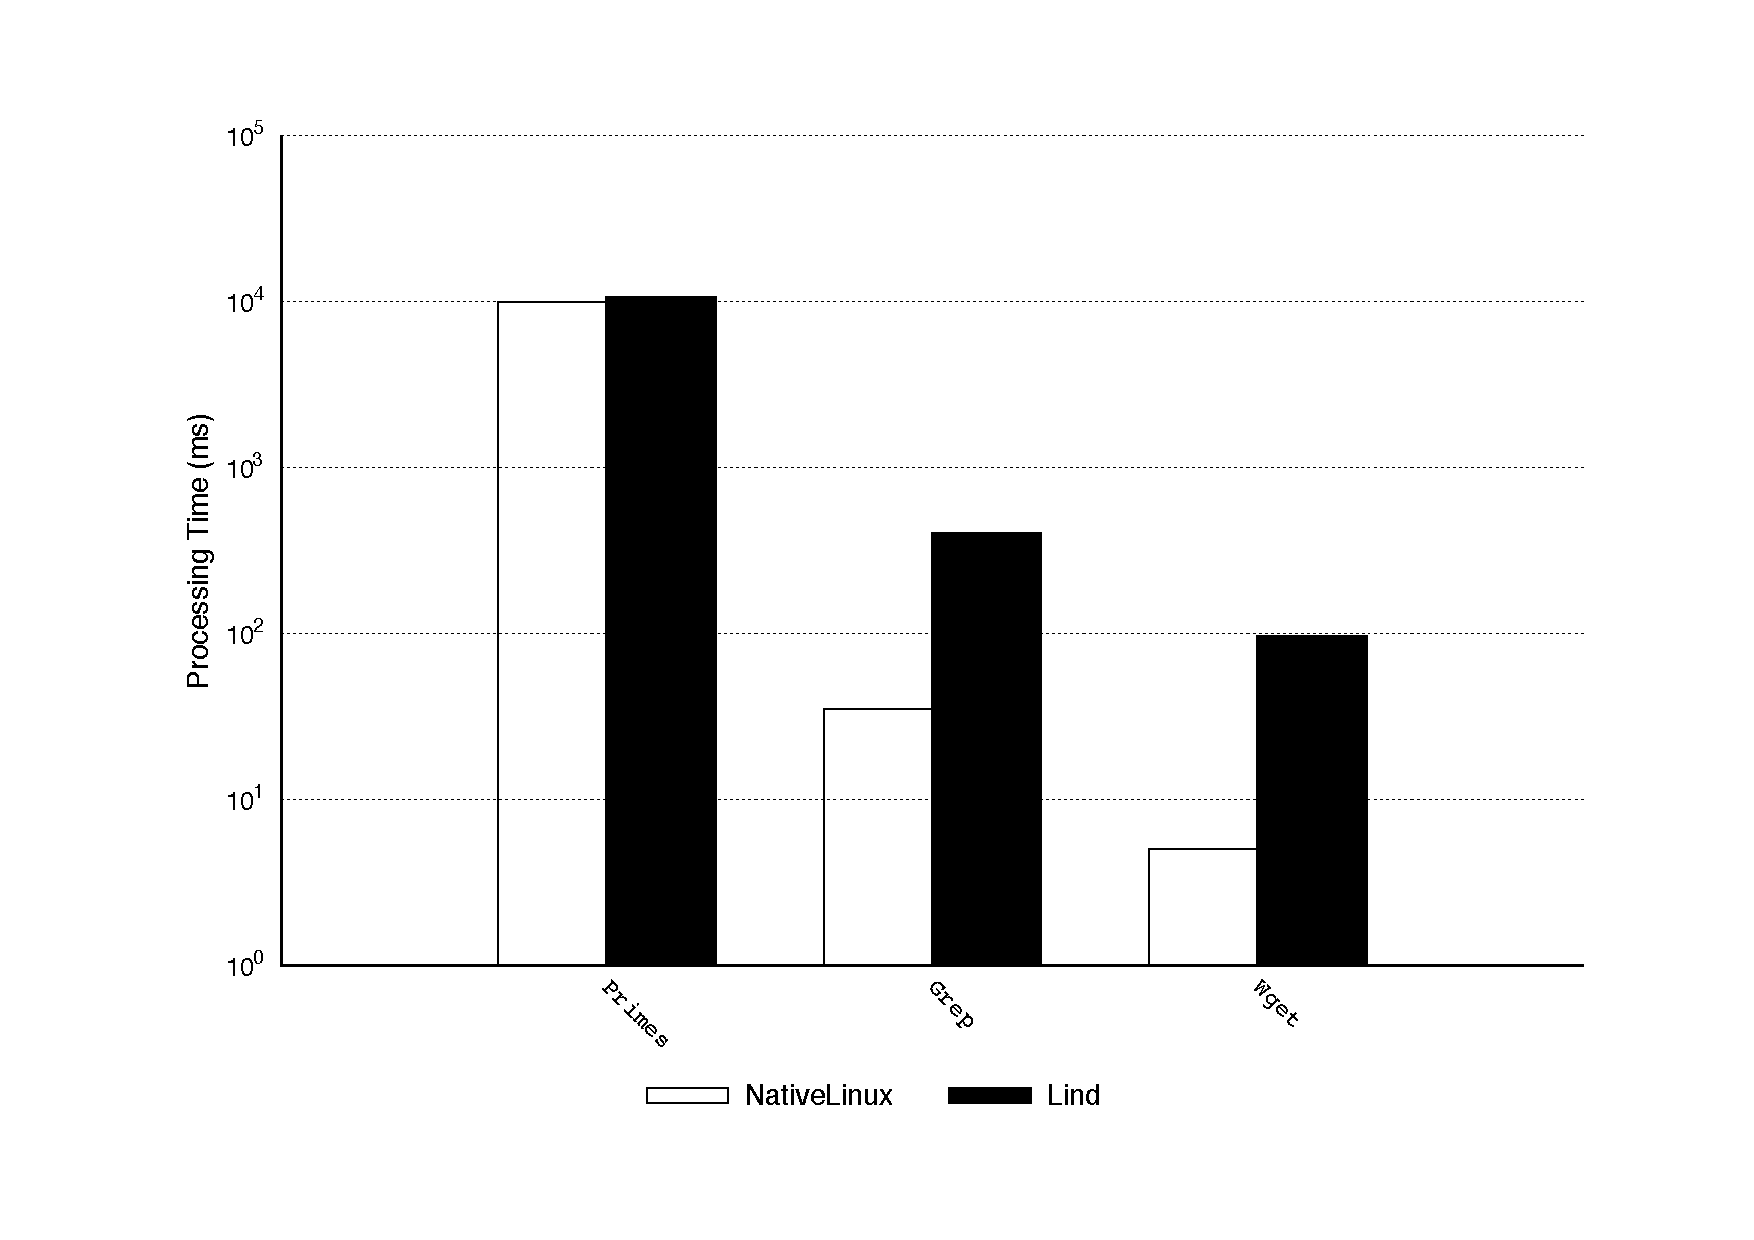
\includegraphics[width=1.0\columnwidth]{diagram/lind_oakland16_performance.pdf}
\caption{\small Overhead from applications run in Native Linux vs. Lind}
\label{fig:performance_applications}
\end{figure}

We evaluated Lind to see
how its performance compared to other systems in a real-world application.
Note that we did not optimize the performance of Lind in any way before running
these tests.

\noindent
\textbf{Setup.}
To test the overhead in Lind for running real-world applications, 
we first compiled and ran three widely used applications:
a prime number calculator, GNU \texttt{grep}, and GNU \texttt{wget}. All ran unaltered and
correctly inside Lind. The source code of each of the applications remained
unmodified. To run the applications, it was sufficient to just recompile the
source code using NaCl's compiler and Lind's \texttt{glibc} to call
into SafePOSIX.

Next, we ran the Tor 0.2.3 in Lind. Tor simply
needs to be recompiled to run in Lind.
We used the benchmarks that come with Tor to test its common operations.

\noindent
\textbf{Results.}
Figure \ref{fig:performance_applications} shows the runtime performance
results for running the primes calculator, GNU \texttt{grep}, and GNU \texttt{wget}. 
The primes application run in Lind has a 6\% performance overhead compared to
Native Linux. CPU bound applications, like the primes, engender little overhead,
because they run only inside the NaCl computation sandbox. No system calls are required,
and there is no need to go through the safe POSIX interface. The small amount of overhead
is generated by NaCl's instruction alignment at building time. Another reason for the overhead
is that the instructions built by NaCl have a higher rate of cache misses, which can slowdown the
program.
We expect other CPU bound processes to behave similarly.
\texttt{grep} experienced roughly 11x slowdown over Native Linux, while \texttt{wget}
slowdown was roughly 19x. Since they are both I/O heavy applications,
each repeatedly calls into the SafePOSIX code which then reimplements
the call.  The additional computation of SafePOSIX produced the additional
overhead. \lois{Is this slowdown significant? Would a slowdown of this magnitude
be acceptable in the real world?}

A summary of the results for Tor is shown in Table \ref{table:performance_tor}. The
benchmarks focus on cryptographic operations,
which are CPU intensive, but also make system calls like \texttt{getpid}, and reads to
\texttt{/dev/urandom}.
The digest operations time the access of a map of message digests.
The AES operations time AES encryptions of several sizes and message
digest creation.
Cell processing executes full packet encryption and decryption. In our
test, Lind slowed down these operations by 2.5x to 5x. We believe these
slowdowns are due to the increased code size produced by NaCl,
%\cappos{I'm not sure why this would be.  Does NaCl show this too?}
and the increased overhead from Lind's safe POSIX system call interface.

As shown above, Lind generally incurs some performance overhead.
It should be noted that, we have not yet attempted to optimize its performance.
However, since an attack on the kernel can have devastating
consequences, %at this initial stage,
a tradeoff between security and performance could be justified.
The fact that Lind is able to run many
\cappos{4 applications isn't many...
Do we have Apache numbers or something else to quantify?}
\yiwen{I am looking at more apps and libs that we can run and test in Lind.}
legacy applications
suggests that it
is a positive step towards building new secure systems.

\begin{table}
\centering
\scriptsize
\caption{\small Performance results on Tor's built-in benchmark program: Native
Linux vs. Lind.}
\begin{tabular}{|r|r|r|r|}
  \hline
  {\bf Benchmark} & {\bf Native Code} & {\bf Lind} & {\bf Impact}  \\
  \hline
  Digest Tests: & & & \\
  Set & 54.80 nsec/element & 176.86 nsec/element & 3.22x \\
  Get & 42.30 nsec/element & 134.38 nsec/element & 3.17x \\
  Add & 11.69 nsec/element & 53.91 nsec/element & 4.61x \\
  IsIn & 8.24 nsec/element & 39.82 nsec/element & 4.83x \\
  \hline
  AES Tests: & & & \\
  1 Byte & 14.83 nsec/B & 36.93 nsec/B & 2.49x \\
  16 Byte & 7.45 nsec/B & 16.95 nsec/B & 2.28x \\
  1024 Byte & 6.91 nsec/B & 15.42 nsec/B & 2.23x \\
  4096 Byte & 6.96 nsec/B & 15.35 nsec/B & 2.21x \\
  8192 Byte & 6.94 nsec/B & 15.47 nsec/B & 2.23x \\
  Cell Sized & 6.81 nsec/B & 14.71 nsec/B & 2.16x \\
  \hline
  Cell Processing: & & & \\
  Inbound & 3378.18 nsec/cell & 8418.03 nsec/cell & 2.49x \\
  (per Byte) & 6.64 nsec/B & 16.54 nsec/B & - \\
  Outbound & 3384.01 nsec/cell & 8127.42 nsec/cell & 2.40x \\
  (per Byte) & 6.65 nsec/B & 15.97 nsec/B & - \\
  \hline
\end{tabular}
\label{table:performance_tor}
\end{table}